% !TeX root = ../cyh.tex

\chapter{starry-next 宏内核}

\section{starry-next 宏内核整体架构}

starry-next (StarryOS) 是构建在 ArceOS 基础之上的操作系统内核。它实现了一个兼容 Linux 的系统调用接口,同时支持多种硬件架构,包括 x86\_64、riscv64、aarch64 和 loongarch64。

代码结构上,starry-next 主要由以下模块组成:

\begin{itemize}
\item core:基于 ArceOS 的底层支持实现 StarryOS 的核心内核功能,包括内存管理(mm)、任务管理(task)和时间管理(time)等。其中内存管理模块负责分配、释放和映射,如 copy\_from\_kernel 函数用于将内核空间的映射复制到用户地址空间,load\_user\_app 函数用于加载用户应用程序到内存中。任务管理模块处理任务和线程的创建、调度和管理,例如 new\_user\_task 函数用于创建新的用户任务。时间管理模块管理系统时间和定时器。
\item api: 现面向用户的 API 和系统调用接口,涵盖文件系统操作、进程管理、线程管理、内存管理等多个方面。
\item src:主要负责启动主函数、加载应用程序并对系统调用的分发进行处理。
\item 其他:包括用于适配不同架构的配置文件和工具链,以及用于构建和运行 StarryOS 的构建工具和脚本。
\end{itemize}

功能上,starry-next 也可以划分为较为独立的模块:

\begin{itemize}
\item 内存管理模块:负责管理物理内存和虚拟内存,包括内存分配、映射和释放等操作。
\item 进程管理模块:负责管理进程和线程,包括进程创建、调度和管理等操作。
\item 文件系统模块:负责管理文件系统,包括文件的创建、读取、写入和删除等操作。
\item 网络模块:负责管理网络操作,包括网络协议栈、网络设备驱动等操作。
\item 系统信息模块:负责提供系统信息和状态,包括 CPU、内存、网络等信息。
\item 信号模块:负责处理信号和中断,包括信号的发送、接收和处理等操作。
\end{itemize}

每个功能模块都需要向应用程序提供相应的系统调用接口,为应用程序提供内核服务。同时,功能模块还需要尽可能复用 ArceOS 的底层组件和接口,以减少代码的重复和维护成本。
功能模块之间通过明确定义的接口进行通信,确保系统的稳定性和可拓展性。

通过结构和功能上的划分与解耦,Starry-next 宏内核的每个模块都可以独立开发、测试和维护,增强了系统的可拓展性和稳定性,也使得本课题大方向上的多名开发者可以在同一代码库上进行协作开发。

\begin{figure}[H]
    \centering
    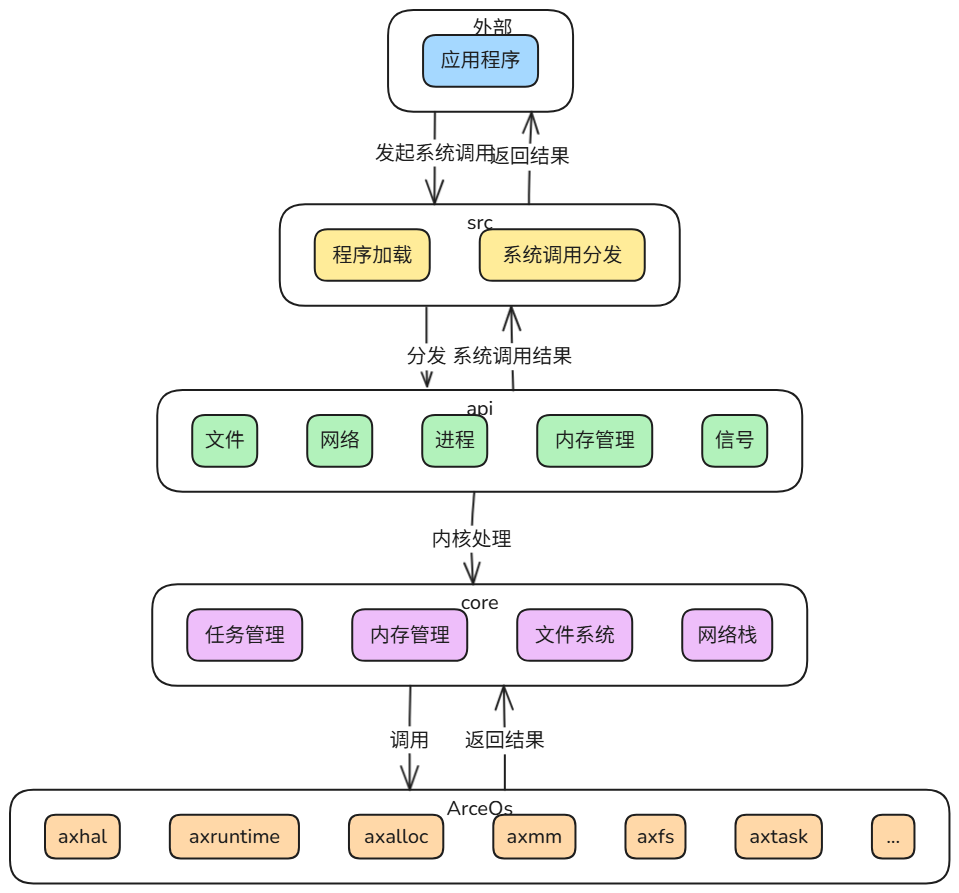
\includegraphics[width=0.7\linewidth, keepaspectratio]{starry-arch.png}
    \caption{starry-next 宏内核架构}
    \label{fig:starry-next}
\end{figure}

\section{starry-next 初始化和运行过程}

% Starry-next 以 main 函数作为系统的入口点,创建初始化进程,为环境变量指定的测试用例创建用户应用程序,并依次运行这些应用程序。在运行过程中,Starry-next 会根据系统资源的需求,动态地分配和管理内存,同时处理各种系统调用,如 fork、exec、wait、mmap、munmap 等。

starry-next 的初始化从 Bootloader 将控制权交给内核入口点开始,之后 ArceOS 的 axhal 模块和 axruntime 模块会完成硬件的初始化,并根据选择的特性进行内存管理器、任务管理器、文件系统、网络等模块的初始化。接着,axruntime 模块以 src 中 main 函数创建一个初始化进程,进而为环境变量指定的测试用例创建用户应用程序,并将用户程序加载到内存中。

% 在运行过程中,starry-next 会根据系统资源的需求,动态地分配和管理内存,同时处理各种系统调用,如 fork、exec、wait、mmap、munmap 等。这些系统调用会使操作系统内核进入内核态,执行 core 中相应的处理程序,并调用底层的 ArceOS 提供的接口进行处理。
% 最后的处理结果将返回系统调用层,进而返回给用户空间的应用程序。

在运行过程中,starry-next 会逐个运行应用程序,并根据系统资源的需求,动态地分配和管理内存。
当应用程序发起系统调用时,先由 src 层将参数根据系系统调用号分发到 api 层的相应处理函数,
api 层的函数会检查参数的类型、取值范围等是否符合系统调用的规范。验证参数无误后,api 层函数会根据系统调用的具体功能,调用 core 层的相关功能模块及其底层的 ArceOS 组件来完成实际的操作。
当 core 层完成操作并返回结果后,api 层会对返回结果进行处理。如果操作成功,api 层会将结果按照系统调用的约定进行封装,以便返回给应用程序。如果操作失败,api 层会根据错误类型设置合适的错误码。
最后,api 层的函数会将处理结果返回给 src 层,src 层会将结果返回给应用程序。

\begin{figure}[H]
    \centering
    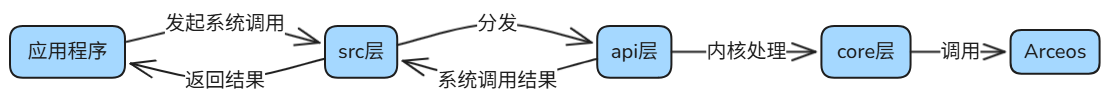
\includegraphics[width=1\linewidth, keepaspectratio]{syscall.png}
    \caption{系统调用流程}
    \label{fig:syscall}
\end{figure}

\subsection{加载程序到内存空间}

在上一节的初始化过程中提到,要运行应用程序,首先需要将其加载到内存空间中。本节将详细介绍 starry-next 是如何加载应用程序到内存空间并执行的。

加载应用程序到内存空间中,首先要创建一个新的用户地址空间,并将内核地址空间的映射复制到用户地址空间,同时映射信号处理的跳板代码。这一步在 run\_user\_app 函数中完成。
接下来,调用 load\_user\_app 函数加载将用户应用程序加载到用户地址空间。该函数使用 axfs::api::read 函数从文件系统中读取用户应用程序的ELF文件数据并进行解析,
如果ELF文件指定了动态链接器(解释器),则递归调用 load\_user\_app 加载。其中,解释器是一种能够将源代码逐行翻译成机器代码并执行的程序,负责加载和解析可执行文件所依赖的共享库。
然后使用 map\_elf 函数将ELF文件中的段映射到用户地址空间中,这一步使用了 map\_alloc 进行的物理页的分配和映射。
最后,分配用户栈和堆空间,并将参数、环境变量和辅助向量(auxv)写入用户栈,返回应用程序的入口地址和用户栈顶地址。

完成程序的加载后,内核会根据用户地址空间创建任务实例,设置任务上下文等相关信息,并将该任务与新的进程和线程关联起来。
最后调用 axtask::spawn\_task 接口将任务添加到任务调度器中,等待调度器调度执行。
run\_user\_app 和 load\_user\_app 函数的流程如图\ref{fig:run-user-app}和\ref{fig:load-user-app}所示。

\begin{figure}
\centering %图片全局居中
%并排几个图,就要写几个minipage
\begin{minipage}[b]{0.3\textwidth} %所有minipage宽度之和要小于1,否则会自动变成竖排
\centering %图片局部居中
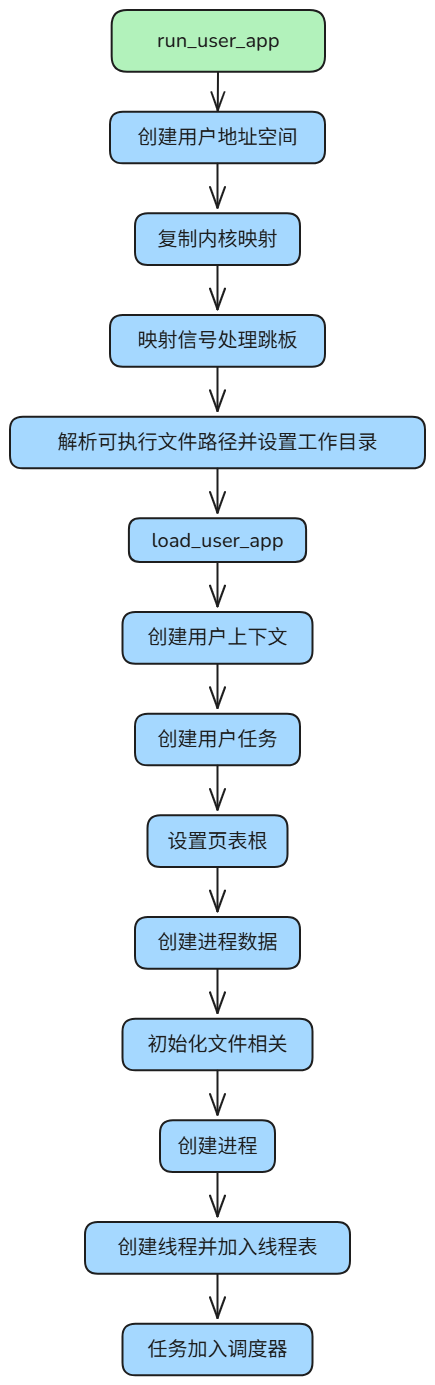
\includegraphics[width=1\textwidth]{run-user-app.png} %此时的图片宽度比例是相对于这个minipage的,不是全局
\caption{run\_user\_app 函数流程图}
\label{fig:run-user-app}
\end{minipage}
\begin{minipage}[b]{0.65\textwidth} %所有minipage宽度之和要小于1,否则会自动变成竖排
\centering %图片局部居中
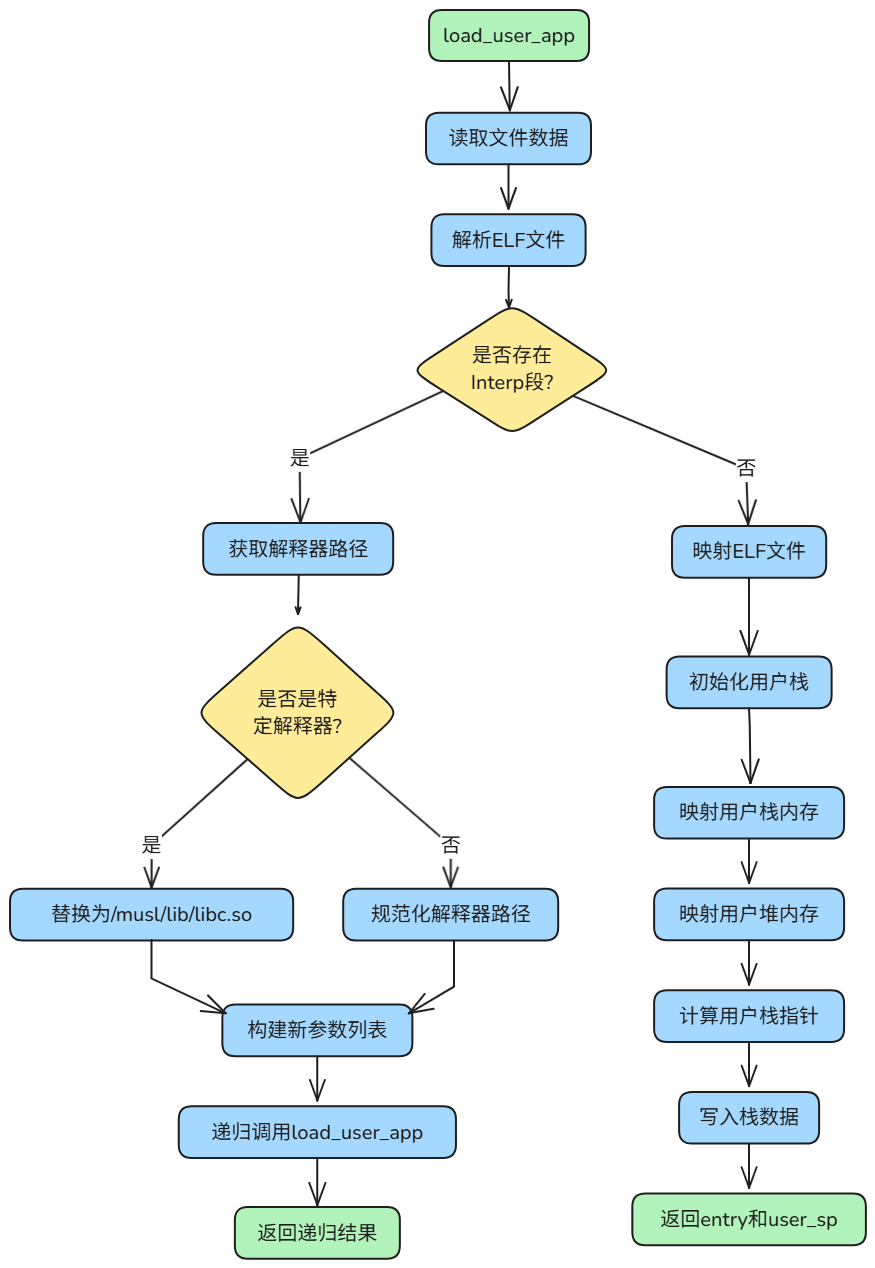
\includegraphics[width=1\textwidth]{load-user-app.png}%此时的图片宽度比例是相对于这个minipage的,不是全局
\caption{load\_user\_app 函数流程图}
\label{fig:load-user-app}
\end{minipage}
\end{figure}


\section{starry-next 内存管理模块}

\subsection{模块结构}

\begin{figure}[H]
    \centering
    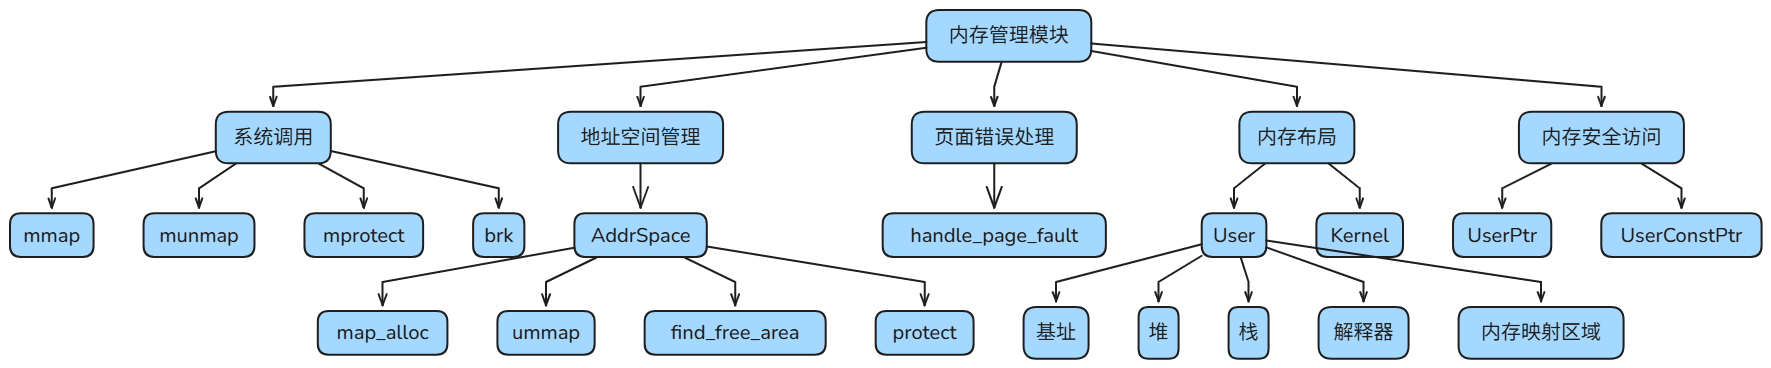
\includegraphics[width=1\linewidth, keepaspectratio]{mm-arch2.png}
    \caption{starry-next 内存管理模块结构}
    \label{fig:mm-arch}
\end{figure}

starry-next 的内存管理模块主要由以下部分组成:

\begin{itemize}
    \item 系统调用:提供了一系列系统调用接口,用于管理内存,如 mmap、munmap、mprotect、brk 等。
    \item 地址空间管理:使用 AddrSpace 结构体及其接口管理用户程序的地址空间,包括内存映射、权限控制等。
    \item 页面异常处理:当用户程序访问内存空间时触发的缺页异常会调用相应的处理函数。
    \item 内存布局:定义了内存布局,包括内核空间和用户空间的划分。
    \item 安全内存访问:通过指针封装提供对用户空间内存的安全访问。
\end{itemize}

\subsection{内存管理机制}

starry-next 的内存管理基本上复用了 ArceOS 的内存管理机制:使用 ArceOS 提供的 AddrSpace 结构体管理用户程序的内存空间,当用户程序需要对内存进行操作时,会调用相应的系统调用,如 mmap、munmap、mprotect、mremap 等,这些系统调用会调用 AddrSpace 结构体的接口在用户地址空间中创建和管理内存映射,同时也会调用全局内存分配器进行物理页的分配和映射。

但作为宏内核,starry-next 需要区分内核态和用户态,因此还对内存管理进行了进一步的优化和扩展,例如为用户态和内核态分别设置了不同的地址空间,并且用户态进程不能直接访问内核态内存空间,
而是需要发出系统调用,通过 trap 机制进入内核态,再进行对应处理,通过这种方式来实现用户态和内核态的隔离;在一些架构中将内核部分的映射复制到用户地址空间,使用户态进程可以直接访问内核的某些数据结构或代码片段,
可以减少内核态和用户态之间的切换开销,提高系统的性能。

\subsection{页面异常处理}
页面异常的处理方面,starry-next 在 ArceOS 的基础上增加了判断:如果是用户态程序访问内存空间或者是内核态程序访问用户内存空间时触发的缺页异常,才会调用用户程序的 handle\_page\_fault 函数,
也就是 ArceOS 的 AddrSpace 结构体提供的页面错误处理函数处理缺页异常,该函数会根据虚拟地址的映射关系,调用全局内存分配器进行物理页的分配和映射。
如果 AddrSpace 结构体不能成功处理该异常,则会打印错误信息并终止当前任务,并发送 SIGSEGV 信号。

\begin{figure}[H]
    \centering
    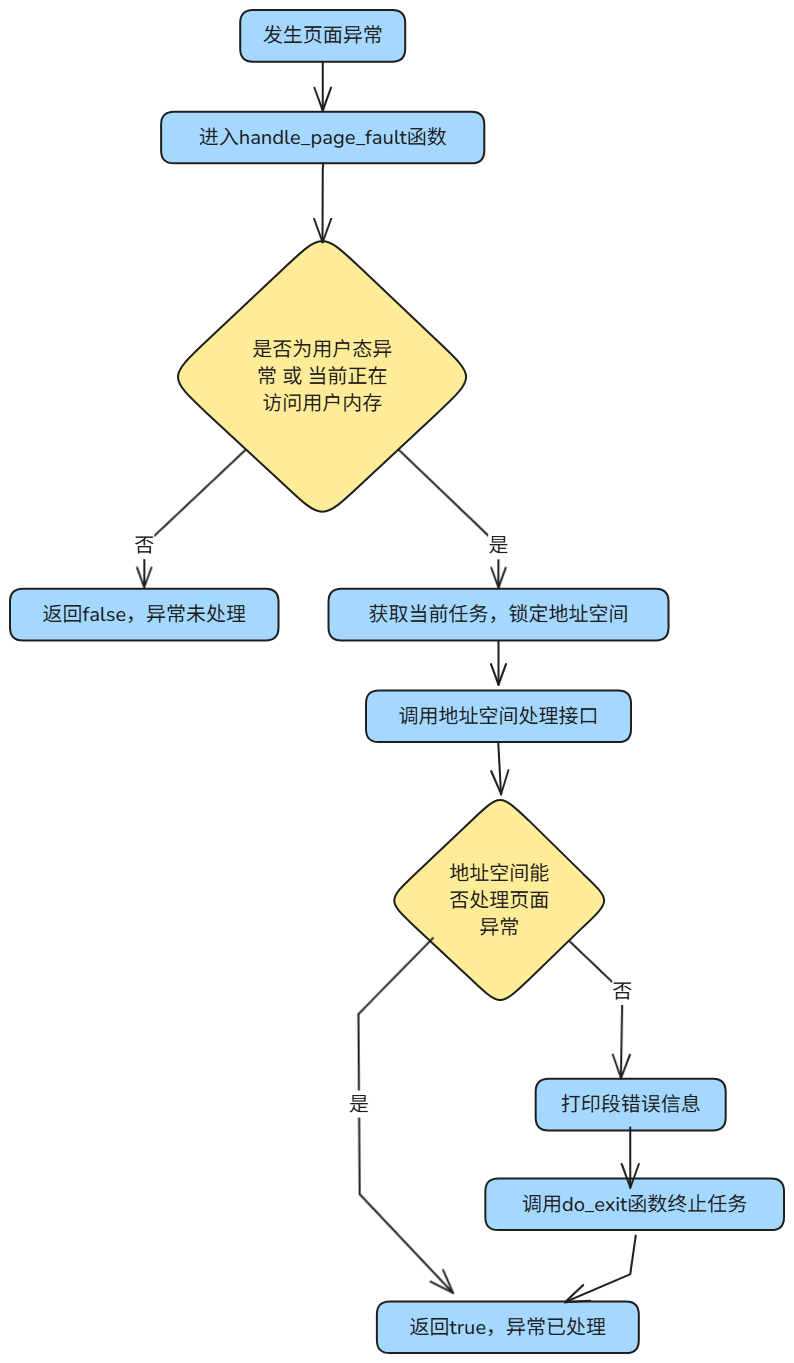
\includegraphics[width=0.7\linewidth, height=14cm,keepaspectratio]{pagefault-starry.png}
    \caption{starry-next 页异常处理}
    \label{fig:pagefault-starry}
\end{figure}

\subsection{内存布局}

不启动 ArceOs 的 paging 特性时,应用和内核在同一空间中运行,系统直接使用物理地址。物理空间的结构如图\ref{fig:phy-layout2}所示。
在 Cargo 项目启动时,axhal 组件的 build.rs 构建文件会根据根据 linker.lds.S 文件中的链接脚本,将物理空间划分为多个部分——内核部分从指定的基地址开始,首先放置可执行代码段(.text),然后是只读数据段(.rodata)和初始化函数数组(.init\_array)。接着是可读写数据段(.data),线程局部存储相关段(.tdata 和 .tbss),以及每个CPU核心的私有数据段(.percpu)。最后是未初始化数据段(.bss),其中包含了启动栈空间,设备内存则位于 0 地址和内核空间之间。整个布局严格遵循4K对齐,并在最后定义了一些与中断处理、系统调用等相关的自定义段。

\begin{figure}[H]
\centering %图片全局居中
%并排几个图,就要写几个minipage
\begin{minipage}[b]{0.45\textwidth} %所有minipage宽度之和要小于1,否则会自动变成竖排
\centering %图片局部居中
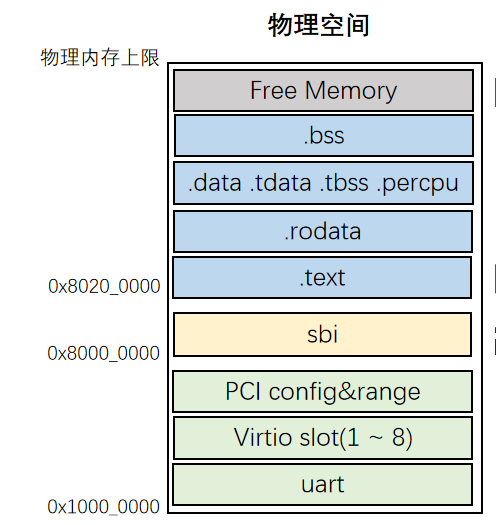
\includegraphics[width=0.8\textwidth]{phy-layout.png} %此时的图片宽度比例是相对于这个minipage的,不是全局
\caption{物理内存布局}
\label{fig:phy-layout2}
\end{minipage}
\begin{minipage}[b]{0.45\textwidth} %所有minipage宽度之和要小于1,否则会自动变成竖排
\centering %图片局部居中
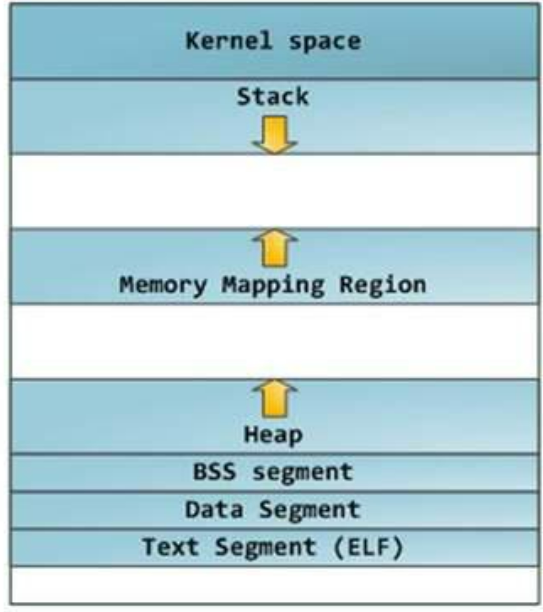
\includegraphics[width=0.8\textwidth]{virt-layout.png}%此时的图片宽度比例是相对于这个minipage的,不是全局
\caption{进程虚拟空间布局}
\label{fig:virt-layout2}
\end{minipage}
\end{figure}


% \begin{figure}[H]
%     \centering
%     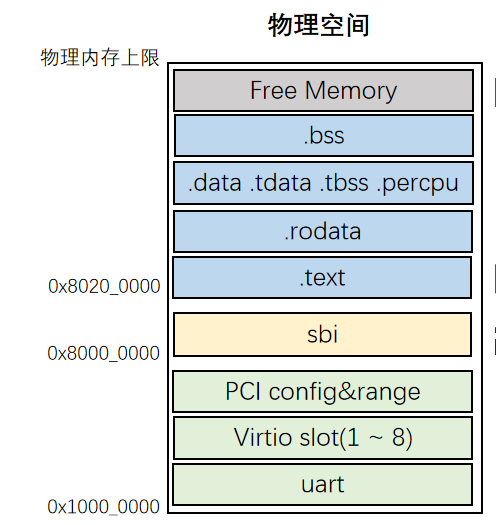
\includegraphics[width=0.5\linewidth, keepaspectratio]{phy-layout.png}
%     \caption{物理内存布局}
%     \label{fig:phy-layout}
% \end{figure}

starry-next 启动了 paging 特性,为每个应用程序分配一个独立的的虚拟地址空间,即 AddrSpace 结构体,用于管理用户程序的内存空间。如图\ref{fig:virt-layout2}所示,进程地址空间分为用户空间和内核空间两部分,用户空间位于低地址,包括了代码段、数据段、堆、栈、内存映射区域。
其中,代码段和数据段是用户程序的只读和读写数据,堆是用户程序的动态内存分配区域,栈是用户程序的函数调用和局部变量存储区域。
内核空间位于高地址,包括了内核代码段、内核数据段、内核堆、内核栈、页表。不同架构下各部分的具体起始地址和大小会有所不同,具体设置可参照表\ref{tab:virt-layout-config}。
% \begin{figure}[H]
%     \centering
%     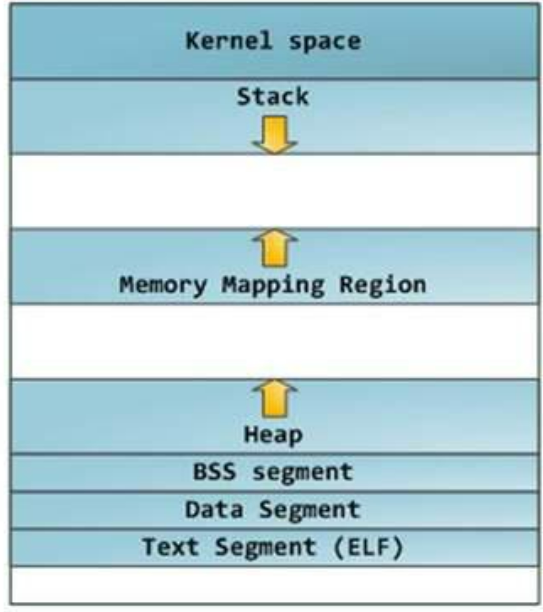
\includegraphics[width=0.5\linewidth, keepaspectratio]{virt-layout.png}
%     \caption{进程虚拟空间布局}
%     \label{fig:virt-layout}
% \end{figure}

\begin{table}[!ht]
    \centering
    \begin{tabular}{lllll}
    \hline
        ~ & x86\_64 & RISC-V 64 & AArch64 & LoongArch64  \\ \hline
        User space base & 0x1000 & 0x1000 & 0x1000 & 0x1000  \\ \hline
        User space size & 128 TB & 4 GB & 128 TB & 4 GB  \\ \hline
        User interpreter base & 64 MB & 64 MB & 64 MB & 64 MB  \\ \hline
        User heap base & 1 GB & 1 GB & 1 GB & 1 GB  \\ \hline
        User heap initial size & 64 KB & 64 KB & 64 KB & 64 KB  \\ \hline
        User stack top & 0x7fff\_0000\_0000 & 0x4\_0000\_0000 & 0x7fff\_0000\_0000 & 0x4\_0000\_0000  \\ \hline
        User stack size & 64 KB & 64 KB & 64 KB & 64 KB  \\ \hline
        Kernel stack size & 256 KB & 256 KB & 256 KB & 256 KB \\ \hline
    \end{tabular}
    \caption{各架构虚拟空间设置}
    \label{tab:virt-layout-config}
\end{table}

\subsection{安全内存访问}

为了保证系统的安全性和稳定性,starry-next 对用户空间内存的访问进行了严格的控制和保护,通过指针封装提供对用户空间内存的安全访问。
具体来说,starry-next 定义了 UserPtr 和 UserConstPtr 两个安全指针类型,分别表示指向用户空间内存的可变和不可变指针。
在访问用户空间内存时,要检查地址是否对齐、当前任务是否有权限访问该地址、地址是否在用户空间范围内并于已经分配映射。
如果这些条件都满足,则可以安全地访问用户空间内存,否则会抛出异常并终止当前任务。

UserPtr 和 UserConstPtr 提供了一系列接口,用于对用户空间内存进行访问和修改。例如:
负责基本信息的查询的 address(获取指针所指向的虚拟地址)和 is\_null(判断指针是否为空)和
获取切片和引用的 get\_as\_mut 和 get\_as\_mut\_slice 等。

\begin{figure}[H]
    \centering
    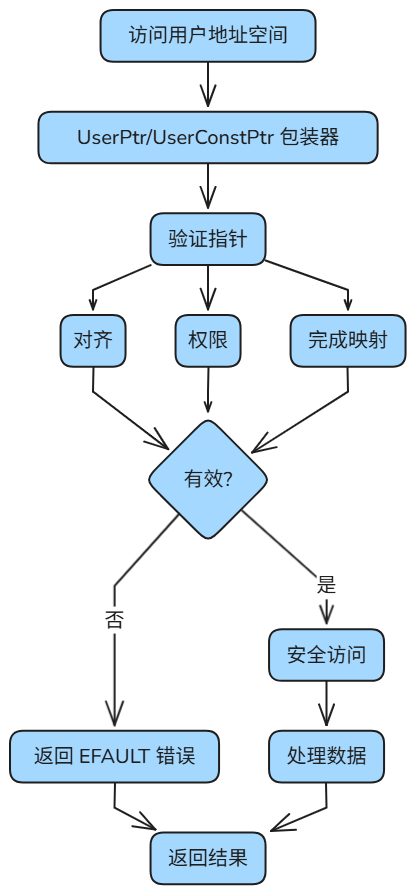
\includegraphics[width=0.5\linewidth]{ptr.png}
    \caption{安全内存访问流程}
    \label{fig:ptr}
\end{figure}